\documentclass[margin = 10pt]{standalone}
\usepackage{xcolor}
\usepackage{tikz}
\usepackage{pgfplots}
\pgfplotsset{
compat = 1.18
}

\begin{document}
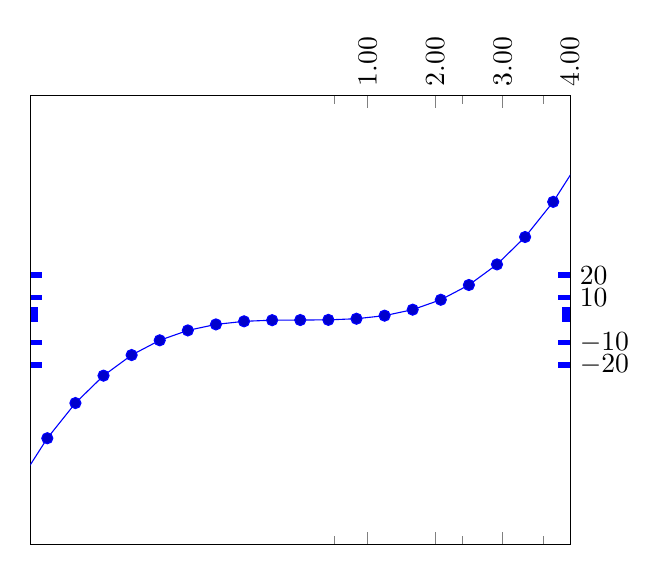
\begin{tikzpicture}[remember picture]
\begin{axis}[
    % 刻度范围
    xmin = -4,
    ymin = -100,
    xmax = 4,
    ymax = 100,
    % xtickmin = -3,
    % ytickmin = -50,
    % xtickmax = 3,
    % ytickmax = 50,
    % 
    % 刻度 数值或标签
    xtick= {1,2,3,4},
    ytick= {-20,-10,10,20},
    ticklabel pos= right,
    % 子刻度
    minor xtick={0.5,2.4,3.6,4.8},
    minor ytick={0.5,2.4,3.6,4.8},
    % 坐标轴刻度样式设置
    % xtick style = {},
    ytick style = {blue,line width = 2pt},
    % tick style = {},
    % 坐标轴数值或标签样式设置
    xticklabel style = {
        /pgf/number format/fixed zerofill,
        rotate = 90},
    ]
\addplot {x^3};
\end{axis}
\end{tikzpicture}
\end{document}